Hensikten med EiT er som nevnt tidligere å forbedre samarbeidsevnene til medlemmer i ett tverrfaglig team ved å anvende sin fagkunnskap i et prosjektarbeid. Det var næringslivet som insinuerte at studentene burde få erfaring i å samarbeide med personer med ulik fagbakgrunn enn dem selv, og at de burde få mer øvelse i å bruke sin fagkompetanse til å løse komplekse oppgaver. Erfaringslæring står i fokus i EiT og utgangspunktet for læringen skal være refleksjon over konkrete arbeidssituasjoner. (\textit{Hva er Eksperter i team (EiT)}?, 2013)\\

I følge seksjon 2.1 hadde gruppas medlemmer mye av de samme forventningene til EiT, men noen vektla visse aspekter mer enn andre. Nedenfor har gruppas medlemmer reflektert over sin personlige utvikling i løpet av prosjektprosessen, samt hvilket utbytte faget har gitt dem.\\

Linn: \textit{''Når jeg ser tilbake på EiT så har det helt klart vært en veldig positiv erfaring å ha med seg videre. Jeg synes det gikk litt tregt i starten med alle øvelsene vi skulle gjøre i plenum, men etter at vi fikk jobbe litt mer selvstendig så har jeg lært utrolig mye om det å jobbe i gruppe. Jeg har blitt mer bevisst på å tilpasse meg andre i gruppa og ser viktigheten av å gi og ta i en gruppe for at dynamikken skal bli så god som mulig. Videre så har jeg holdt på mye med det tekniske, altså programmering av PHP, javascript, HTML og CSS og føler jeg har lært en del der. Selv om det jeg har lært aller mest av er at det er viktig å reflektere over det man gjør i gruppa, snakke sammen og planlegge for å oppnå et godt resultat.''}\\

Silje: \textit{''EiT har gitt meg mye ny erfaring og kunnskap. Selve arbeidet med prosjektet og koblingsagenten har medført at jeg har tilegnet meg ny terminologi innenfor tekniske områder som MySQL, PHP, Github og Javascript. Likevel er det selve prosjektprosessen som har gitt meg mest lærdom. Jeg føler at jeg har blitt mye mer bevisst på hvordan jeg oppfører meg og hvordan jeg bør oppføre meg i en gruppe for å ende opp med best mulig resultat. Det har vært veldig lærerikt med den ulike fasiliteringen fordi den har gjort oss klar over situasjoner som ellers ville gått upåaktet hen. Alt i alt har min EiT-opplevelse vært positiv, og jeg tror absolutt at faget har forbedret mine samarbeidsevner.''}\\

Espen: \textit{''I løpet av prosjektets gang har jeg blitt tilført mange nye erfaringer. I hovedsak har disse erfaringene omhandlet hvordan jeg som gruppemedlem blir oppfattet av andre. I den anledning har faget gitt meg bedre selvinnsikt, og har ført til at jeg har gjort endringer for å bedre gruppa som helhet. Jeg føler også at EiT har gjort meg mer bevisst på hvordan man kan evaluere andre, og hvordan man skal fremstille disse observasjonene på en god og konstruktiv måte. Videre har faget gitt meg faglig kunnskap innenfor emner jeg ikke besatt før, spesielt relatert direkte til koblingsagenter. I sin helhet har emnet brakt med seg et meget positiv inntrykk, og jeg føler helt klart at mine opprinnelige mål har blitt oppfylt.''}\\

Per: \textit{''EIT har for meg vært en positiv opplevelse, hvor jeg har lært mye om gruppedynamikk og hvilke faktorer som er viktige for at en gruppe skal fungere bra. Videre har jeg også blitt mer bevisst på hvordan andre opplever meg som et gruppemedlem og hva jeg kan gjøre for å være et best mulig gruppemedlem. Det har også vært en god leksjon i evaluering av meg selv og evaluering av andre på gruppa. Faglig har jeg fått en oppfriskning av webspråk og lært en god del om hvordan man kan skrive koblingsagenter som er kosteffektive til riktig formål, med tanke på tid det tar å utvikle, skalerbarhet, utviklingspotensial osv.''}\\

Mats: \textit{''I utgangspunktet var jeg noe skeptisk til EiT og opplegget, basert på hva jeg hadde hørt fra andre, og det generelle førsteinntrykket jeg fikk. Dette viste seg fort å være ubegrunnet skepsis, da jeg har opplevd opplegget som positivt. Jeg har blitt mer bevisst på hva som definerer godt gruppesamarbeid og tiltak som kan gjøres for å videre fremme samarbeid.  Selv føler jeg at jeg har hatt en personlig utvikling under EiT prosjektet, da jeg spesielt har fått noe innsikt i hvordan andre gruppemedlemmer oppfatter meg. Jeg har også fått ett noe annet syn på hvordan åpenhet kan påvirke samarbeid generelt i en positiv retning. Jeg har også lært noe av programmeringsspråket PHP, for utvikling av web-baserte applikasjoner.''}\\

Basert på disse refleksjonene kan vi konkludere med at gruppemedlemmene overordnet sett har hatt et positivt inntrykk av EiT. Alle påpeker at de har fått ny, faglig innsikt, men at det er refleksjonene rundt selve prosessen som har gitt dem mest ny kunnskap. En ordsky (fig. XX) er generert med utgangspunkt i de personlige refleksjonene for å illustrere hva som er gjennomgående i gruppemedlemmenes refleksjoner. Ordskyen kan indikere fellestrekk i gruppemedlemmenes oppfatning av læringsutbytte i faget som igjen kan sammenliknes med fagets læremål.\\

\begin{center}
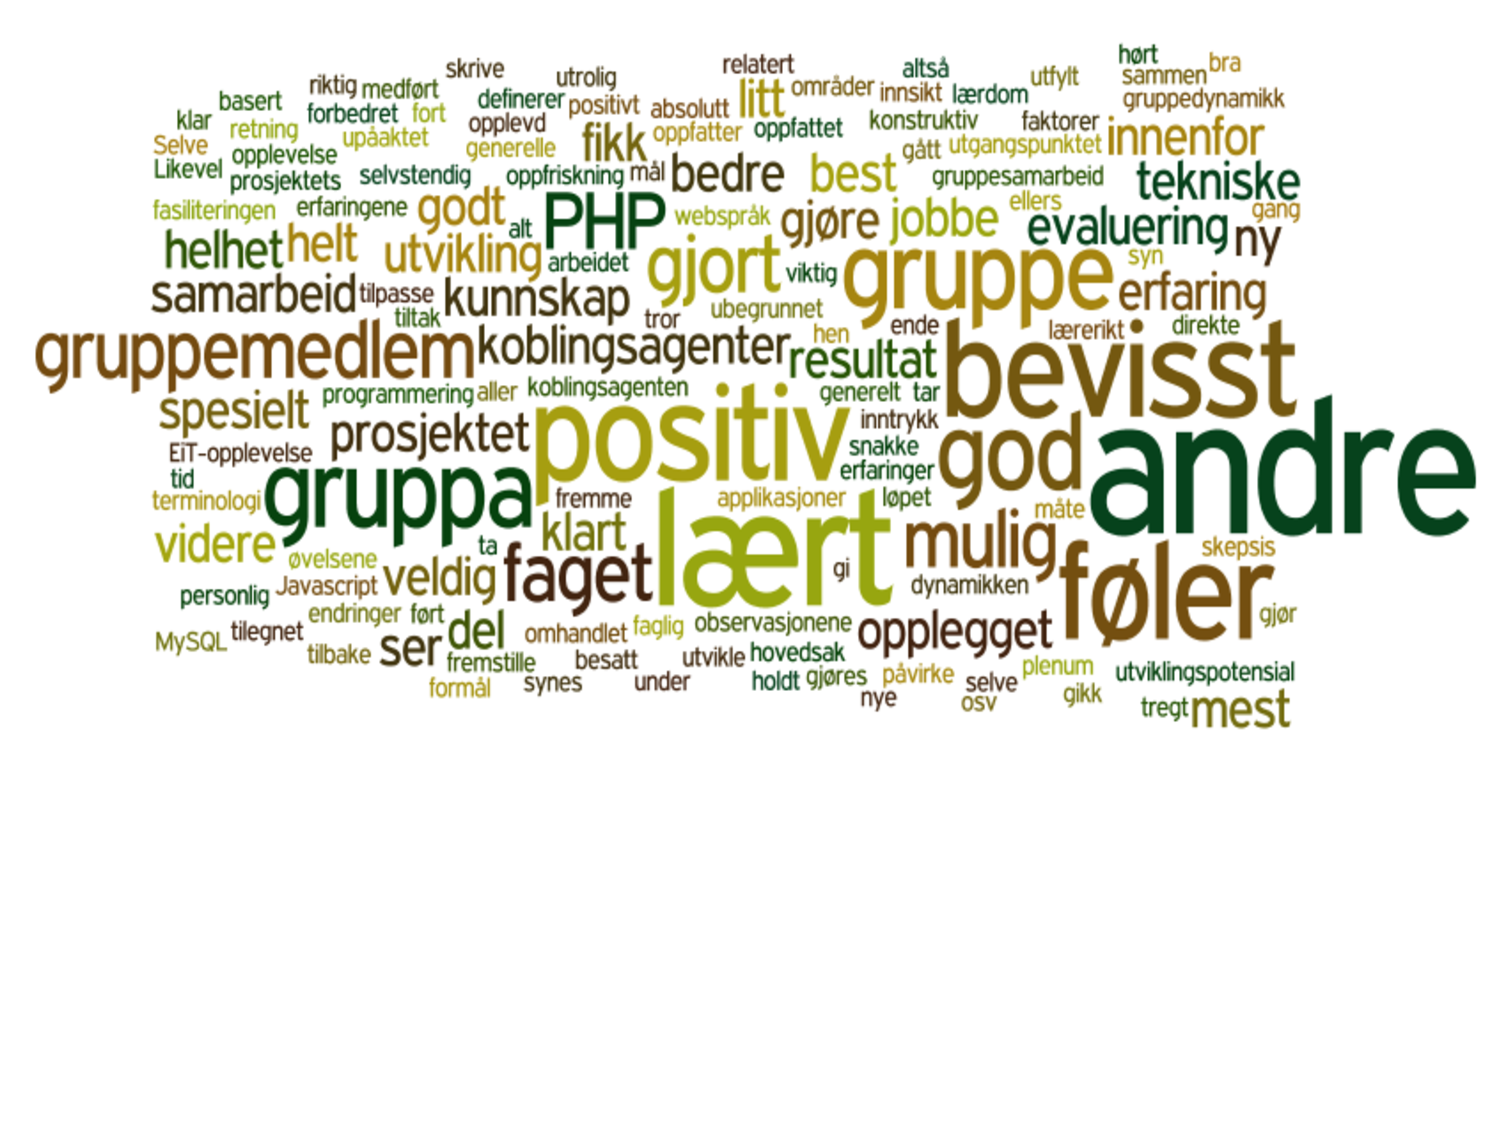
\includegraphics[clip=true, width=1 \textwidth,
trim=0cm 0cm 0cm 0cm]{ordsky.pdf}
\captionof{figure}{Ordsky generert av refleksjoner}
\label{fig:Ordsky}
\end{center}

Ordene \textit{andre, positiv, bevisst, gruppe/gruppa, lært, føler og PHP} skiller seg ut som noen av de mest brukte ordene. Dette resultatet bekrefter tidligere påstander om at gruppemedlemmene generelt sett har ett positivt inntrykk av EiT og at prosessen og samarbeidet har stått i sentrum. Av de 8 mest brukte ordene er det kun ett av de som omhandler den tekniske biten av arbeidet; PHP, mens mange omhandler selve samarbeidsprosessen. Spesielt ordet bevisst skiller seg ut. Dette tyder på at gruppemedlemmene føler at de har blitt mer bevisst på ulike aspekter ved gruppearbeid, noe som går igjen i flere av fagets læremål.\\

Alt i alt, kan vi konkludere med at gruppa har lært mye i løpet av prosjektperioden og flere av læremålene er tilsynelatende oppfylt.\\
